\chapter{Network flexibility and consistency across tasks}

\section{Motivation}

Is cognitive flexibility mirrored by functional network flexibility? That's the question we are now led to ask. In Study 1, we established that the degree of global modularity -- a key component of an efficient small-world architecture -- at rest is positively associated with reading skill. The exception to this was in the cingulo-operculuar and auditory networks, which had a negative correlation; that is, lower segregation of these areas was associated with better reading. In Study 2, we found that reading comprehension induced a more integrated network architecture as information was shared across RSNs. However, the relationship between reading skill and modularity persisted, even as connectomes were estimated during separate conditions. 

Thus, it appears that flexibility in functional networks -- at least those constructed using functional MRI -- across different tasks may not be related to efficiency of cognitive processing. Rather, better readers seem to have a shared and strong network ``backbone'' that is persistent throughout task reconfiguration. One way to test this in the context of reading would be to quantify the degree of reconfiguration (or conversely, similarity) between the task-evoked architecture. Given that reading is a skill that we know requires a very high degree of cross-RSN interaction, we might expect this to be true in a variety of other domains as well. In fact, we might expect that there would be a high degree of consistency between a number of different tasks: listening and reading, but also more basic attention and resting states. 

In this third study, we expand our task and analyses to encompass the auditory modality in order to address two questions. First, do better readers have greater similarity between different language comprehension conditions? Second, to what extent does flexibility in network organization predict individual differences in reading skill and cognition? Below, we motivate these two aims individually.

\subsection{The connectome in language comprehension}

The most widely-held view is that reading and listening share the same core linguistic processes and differ primarily in the sensory processes that feed into supra-model linguistic systems \citep{Mattingly1971, Price2012}. One popular model, the \textit{Simple View of Reading} states that reading comprehension is the product of listening comprehension and decoding skills \citep{Gough1986}. This view has received support from large behavioral studies \citep{Kirby2008} and neuroimaging investigations: many of the literacy-related changes are linked to visual or phonological systems, areas not directly related to semantic or comprehension processes \citep{Schlaggar2007, Dehaene2015}. These findings support a model in which inputs from auditory or visual domains are fed up into higher-order association areas that sequence, encode articulation plans, and extract semantic information \citep{Price2012}. These processes localize onto the similar areas regardless of language and writing system \citep{Rueckl2015}, and may even extend to inputs from somatosensory domains \citep{Xu2005, Sood2016}. This supra-modal language core is largely left-lateralized and centers on the inferior frontal gyrus, anterior and posterior middle temporal gyrus and the angular gyrus. Neuroanatomical models of language, for example the one shown in Figure \ref{fig:ch4-price-language-models}, illustrate that language is distributed throughout much of the brain with a high degree of overlap between listening and reading comprehension. 

\begin{figure}[t]
	\centering
	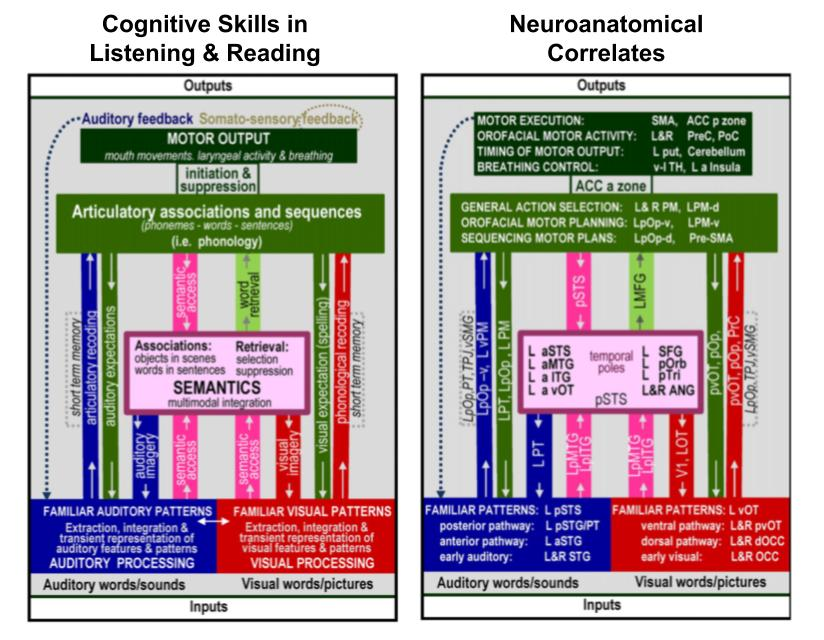
\includegraphics[width=6in]{ch4-price-language-models}
    \caption[Common core architecture for reading and listening]{There exists a common core architecture for reading and listening. The models presented here contend that reading and listening share the same core processes, with the major differences being in the sensory processing functions. Figure adapted from \citep{Price2012}.}
	\label{fig:ch4-price-language-models}
\end{figure}

Most cognitive models suggest that language comprehension requires the construction of a mental representation that includes textual information and associated background knowledge, connected by some conscious and some unconscious executive processes \citep{Kendeou2014}. During comprehension, the relationship between areas is dynamic and constantly being re-evaluated. The roles of attention and executive systems are likely to play an important role. Thus, while there may be a core set of systems for manipulating and extracting meaning from language, it is likely that differences in modality would modulate these processes. 

Despite the clear overlap between reading and listening, there is also evidence that the two skills are not directly equivalent. The pioneering researcher Alvin Liberman suggested that reading is parasitic on listening: it requires the majority of the listening machinery, as well as an awareness of the linguistic act \citep{Mattingly1971}. There is a subset of students who, despite adequate word decoding skills and vocabulary skills, struggle with reading comprehension \citep{Pimperton2010, Spencer2014}. From a neurobiological perspective, expected differences in primary visual areas (for reading) and primary auditory areas (for listening) represent the different input systems, with ventral occipito-temporal systems also activating \citep{Jobard2007}. However, differences in core language systems are also observed: additional activation in left posterior temporal and parietal areas in reading modality \citep{Constable2004}, as well increased bi-laterality especially in children \citep{Berl2011}. Altogether, there is substantial evidence that reading relies on existing speech comprehension circuitry. Therefore, a \textit{convergence} in the evoked networks may be an indicator of better reading.

\subsection{The connectome across many tasks}

As seen in Chapter 3, global and regional network architecture changes during task activation, but it preserves its overall modular structure nonetheless \citep{Cole2014}. A subsequent question is, what attributes of the network architecture enable flexibile reorganization while also preserving modularity? Strong candidates for this role are hub regions, but these should also show flexibility across a number of tasks -- not just listening and reading but other cognitive tasks as well. 

The ``flexible hub'' theory asserts that a subset of regions in the brain are responsible for coordinating other brain systems in the accomplishment of internally-directed aims \citep{Cole2007}. Hubs provide a way in which the brain might maintain its overall modular architecture while still increasing communication between regions. While there are a number of cognitive systems that may perform hub-like functions, including the salience, dorsal attention, ventral attention, and cingulo-opercular networks, several researchers have targeted the front-parietal network as a particularly important set of areas likely to perform hub-like functions \citep{Cole2013, Niendam2012}. 

The frontoparietal network is an assembly of brain regions encompassing the lateral frontal and parietal cortices along with insular, anterior/mid cingulate, and inferior temporal areas that have been broadly implicated in a variety of higher-level cognitive tasks \citep{Fedorenko2013}. One reason it has been targeted is that it encompasses the lateral prefrontal cortex, which has been seen to exert top-down control over other brain areas and which is often active in novel or difficult tasks \citep{Duncan2010}. Some have described the frontoparietal network as supporting active and adaptive online control, initiating and adjusting goal-directed mental systems \citep{Dosenbach2007}, while others have proposed a more general superordinate role in directing cognition \citep{Niendam2012}.  Global functional connectivity in the fronto-parietal network has also been shown to predict individual differences in cognitive skills and intelligence \citep{Cole2011}. Taken together, there is significant evidence for the importance of hub regions in supporting flexible cognition, and the fronto-parietal network may be particularly important. 

\subsection{Study aims}

On the one hand, we have evidence that modularity within the global network, in any condition, is predictive of reading skill. On the other hand, we know that different skills rely on different brain areas and require different systems to coordinate. Therefore, the aims of the present study were to determine to what extent flexibility across different tasks is predictive of individual differences in skilled reading.  First, we test \textit{similarity} between listening and reading network architecture corresponds to higher reading skill. Second, we examine whether \textit{dissimilarity} among resting-state networks across many conditions will correspond to higher reading skill (that is, variability in connectivity). We expect that this dissimilarity will be most present in associative RSNs such as the fronto-parietal network. 


\section{Methods}

\subsection{Participants}

Participants were drawn from the same cohort of subjects included in Studies 1 and 2, and identical inclusion criteria for both demographic and scan motion were applied. However, additional measures related to the performance of the task were levied as described below. A total of 42 unique subjects and 142 scan sessions were included in the analysis. The demographics for these subjects are described in Table \ref{table:ch4-participants}.

\begin{table}[t]
	\renewcommand{\tabcolsep}{0.09cm}
	\centering
	\begin{tabular}{lc}
\toprule
Measure &               Value \\
\midrule
Subjects                        &              42 \\
Mean age                        &    10.51 (0.33) \\
Sex                             &      21 M, 23 F \\
WASI Full-Scale IQ, Vocabulary  &    52.91 (9.38) \\
Test of Word Reading Efficiency &  104.66 (18.07) \\
\bottomrule
\end{tabular}
	\caption[Participant demographics for Study 3]{Participant demographics for Study 3. Participants were a subset of those examined in Study 2, who had also completed a listening comprehension task with sufficiently high quality.}
	\label{table:ch4-participants}
\end{table}

\subsection{Functional MRI acquisition and processing}

The task design for this study is described in detail in Chapter 3. Briefly, subjects were presented up to four separate runs of a language comprehension task. The task included two passage blocks (``reading'' or ``listening''), two sensory baseline blocks (``symbols'' or ``tones'') and a trailing resting-state block (``rest''). The four scan runs were crossed on two conditions: the modality of presentation (auditory or visual) and the genre of the passage (narrative or expository). 

A scan session was excluded based on the following parameters: the number of high-motion volumes exceeding 20 percent, mean frame-wise displacement greater than 0.4, or poor task performance ($D^\prime < 2$). To control for the effects of genre, we matched all scans that met inclusion criteria with their opposing-modality counterpart, so that each subject had either 2 scans (same genre in listening and reading) or 4 scans (both genres in listening and reading). In total, 42 children (142 scans) met inclusion criteria.

Functional MRI acquisition and preprocessing procedures were equivalent to those described for Study 2. See the \textit{Methods} section of Chapter 3 for a detailed description of these processes and their parameters.

\subsection{Activation and network analyses}

Our analysis was broken into two parts: first, comparing the similarities and differences in network organization for listening and reading, then across all available tasks. 

For the modality comparisons, we used a fixed-effects subject-level model to estimate the shared activation for ``listening and reading'' and their differences ``listening vs. reading''. We then used FSL's \textit{randomise} utility to estimate the main effects of modality across all subjects in our sample (5000 permutations, threshold-free cluster enhancement, $p < 0.05$).  We also investigated these effects in ``connectome space'' by extracting the values at each of the 264 nodes used for connectivity analysis, then comparing the activity profile of each RSN during reading and listening.

\subsection{Network similarity estimation}

Global modularity estimates the similarity of a network to a reference partition, such that two networks with high modularity must be similar to the reference, but not necessarily to each other. This method, while useful, has the drawback of being biased towards the provided RSN parcellation: two networks could receive the same modularity score, but deviate in significant ways (i.e. both similar to partition but not to each other). 

\begin{figure}[t]
	\centering
	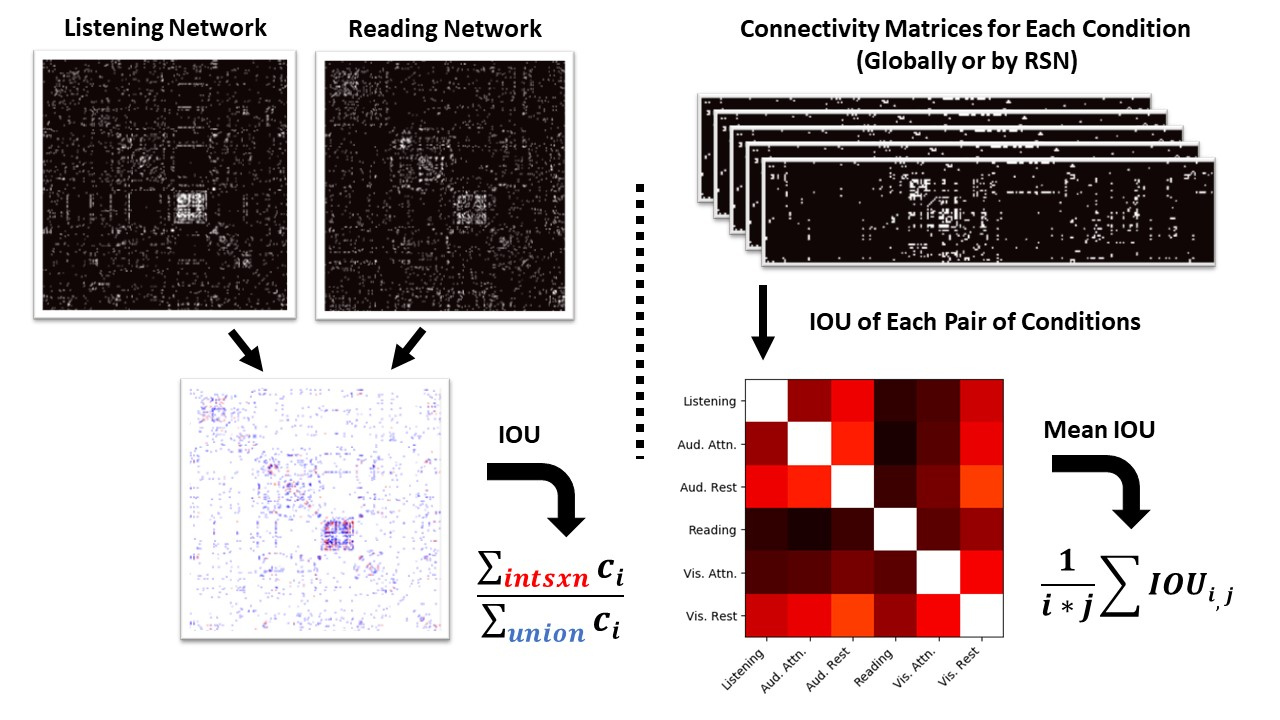
\includegraphics[width=6in]{ch4-network-similarity-methods}
    \caption[Methods for measuring similarity between whole-brain connectomes]{Schematic of methods for measuring similarity between whole-brain connectomes. The intersection of the union (IOU) can compare two connectivity arrays without reference to a pre-defined set of RSNs. On the left are methods for comparing listening to reading connectomes. On the right are methods for comparing, for each whole-brain network or RSN array, the similarity across all all task and rest conditions.}
	\label{fig:ch4-network-similarity-methods}
\end{figure}

One similarity metric that is not biased towards a reference is the \textit{intersection of the union} (IOU). To calculate the IOU of two binary matrices, one sums the total number of shared connections (intersection) and divides it by the total number of connections in either array (union), resulting in a value between 0 to 1, with 0 corresponding to no shared connections and 1 representing identical arrays. IOU provides two advantages compared to simply calculating the number of shared connections: it converts all comparisons to a common range, and it can compare arrays with different numbers of connections without being biased towards dense arrays (e.g. comparing an array with many connections to one with few connections). The IOU approach provides a complementary perspective to estimates of modularity.

We first compared the IOU of network arrays across individuals within the two linguistic conditions: listening to listening and reading to reading. We summarized the distributions of the IOU, with the expectation that there would be the most variability within the reading condition, since listening is more ``natural''. Next, we tested whether the similarity between an individual's reading and listening network arrays was related to reading skill. Finally, we analyzed RSN-level patterns of similarity and difference between reading and listening. 

Next, we broadened the scope of analysis to include comparisons between all task conditions: rest (x2), symbols, tones, listening and reading. For each subject, we calculated the IOU between each evoked network in all conditions. This resulted, for each subject, in 15 network comparison values, for each set of nodes examined. The question we were interested in was whether, within-subject, individuals who had fewer changes in network configuration were also better cognitive performers. We then sought to determine whether changes within a single RSN (e.g. the fronto-parietal network) were the key drivers of this. 


\section{Results}

\subsection{Behavioral results}

Attention and comprehension measures were not related to modality of stimulus presentation. There was a trend towards difference in median FDRMS between scan modalities (paired t-test, $t = 1.904$, $p = 0.059$), so we also replicated analyses with a stricter motion threshold (no more than 10 percent outliers in a scan run). The main results from analysis of this 35 subject (116 scan runs) cohort were broadly consistent.

\subsection{Activation results}

As expected, reading and listening shared a common core of language-related activations. These included the bilateral middle temporal and inferior frontal gyri, as well as the  anterior temporal poles. The differences related to modality fell into three categories: sensory processing areas, including the insula, superior temporal gyrus, and secondary visual processing areas; and hetero-modal association areas, most notably the inferior frontal gyrus and angular gyrus; and somato-motor regions, including the premotor cortex and lateral geniculate nucleus of the thalamus (Fig. \ref{fig:ch4-modality-comparison-attn}). Areas showing greater activation in listening localized on primary auditory cortex and the dorsal attention network.

\begin{figure}[t!]
	\centering
	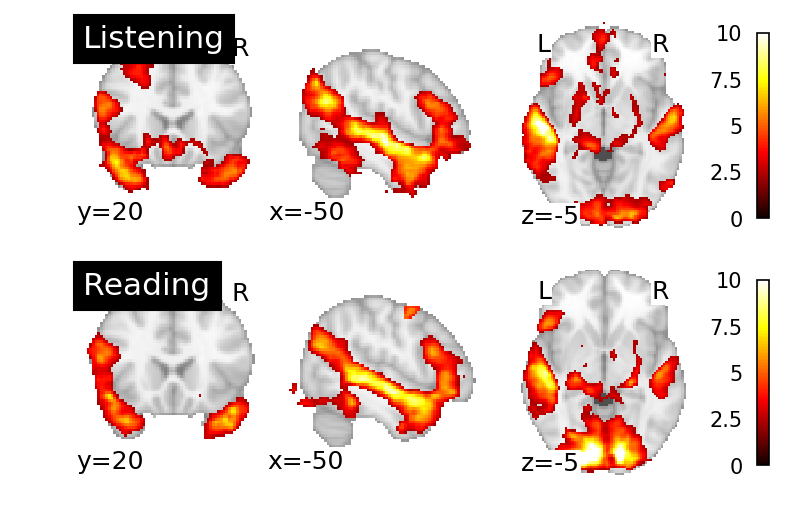
\includegraphics[height=3in]{ch4-modality-comparison-attn}
	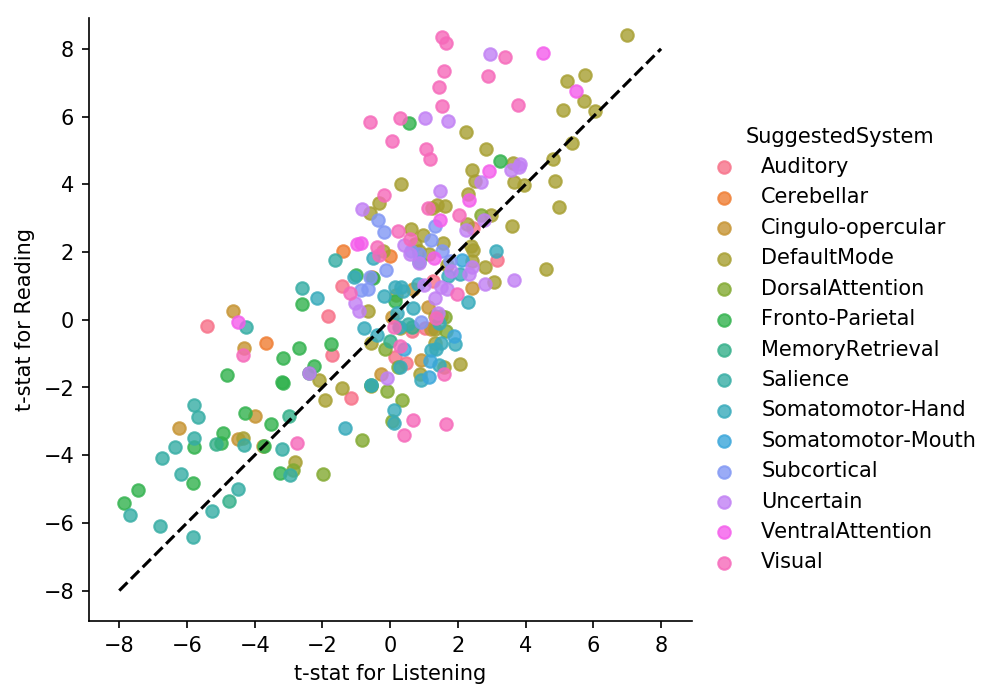
\includegraphics[height=3in]{ch4-listening-reading-connectome-activation-attn}
    \caption[Large overlap between listening and reading activation]{There was a large overlap in activation between the listening and reading comprehension tasks. Activation spanned a bilateral set of regions, especially around middle temporal, inferior frontal gyri. Activations shown for $p < 0.05$, threshold-free cluster enhancement (5000 permutations).}
	\label{fig:ch4-modality-comparison-attn}
\end{figure}

This result is more easily visualized when viewing it in terms of the 264 nodes of the connectome. There was a very high correlation coefficient between activation during reading and listening compared to the sensory baseline ($r = 0.748$, $p < 0.001$), reflecting the high degree of shared activity in the language network. Relative to rest, the variability was slightly higher ($r = 0.552$, $p < 0.001$), but still significant. 

In general, areas that are active during listening are also active during reading, but there were differences in the intensity with which they were activated: many nodes were more strongly activated in reading compared to listening. Figure \ref{fig:ch4-listening-reading-network-activation-attn} displays these in connectome space. These fell predominantly into the ventral attention, visual, and default mode networks. Only a few areas were more active in listening than reading: areas in the dorsal attention network and a few in the default mode and salience networks. 

\begin{figure}[t]
	\centering
	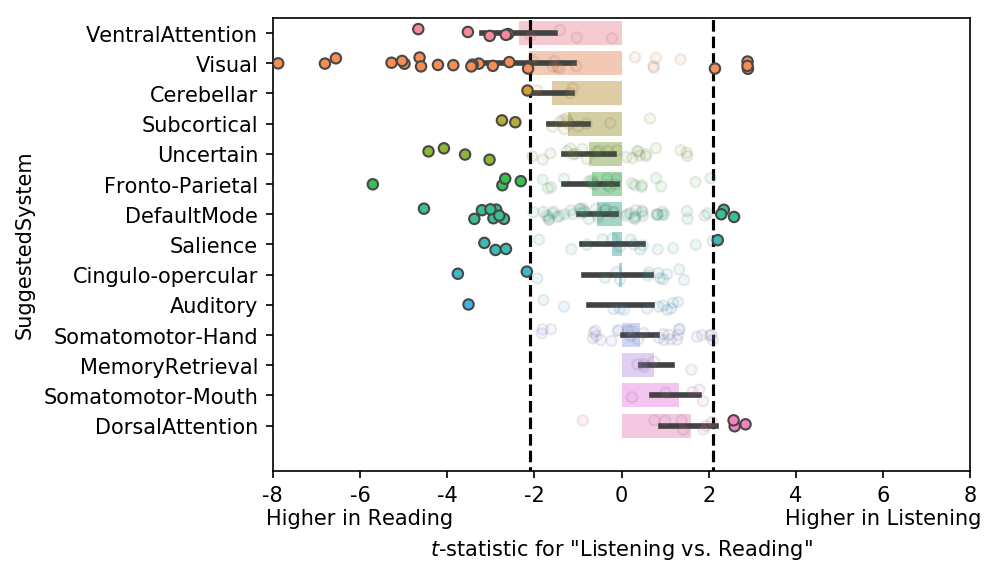
\includegraphics[height=3in]{ch4-listening-reading-network-activation-attn}
    \caption[Activation differences due to modality of presentation among RSNs]{Activation differences due to modality of presentation among RSNs, when both tasks were compared to their sensory baseline. Each point represents a single node, while bars represent the aggregate mean for each RSN. Visual and ventral attention networks showed the most network-level activity in reading, although large portions of the default mode and fronto-parietal network were also robustly related. Cingulo-opercular, memory retrieval and salience networks showed decreases. Dashed lines represent $p < 0.05$, uncorrected.}
	\label{fig:ch4-listening-reading-network-activation-attn}
\end{figure}

\subsection{Network results}

In terms of graph theory measures, we found a significant decrease in modularity ($t = 3.670$, $p < 0.001$) and a significant increase in participation coefficient ($t = -4.312$, $p < 0.001$) in reading compared to listening (top panel of Figure \ref{fig:ch4-modality-graph-theory}). Investigating the differences in path length between the two modalities provides a stronger sense of key drivers of this increased integration. The bottom panel of Figure \ref{fig:ch4-modality-graph-theory} displays the node-level connections of nodes that get closer or further during the reorganization. The large amounts of red reflect the greater global integration seen in reading; the blue patches represent a reduction in modularity within visual networks especially.

\begin{figure}[t!]
	\centering
	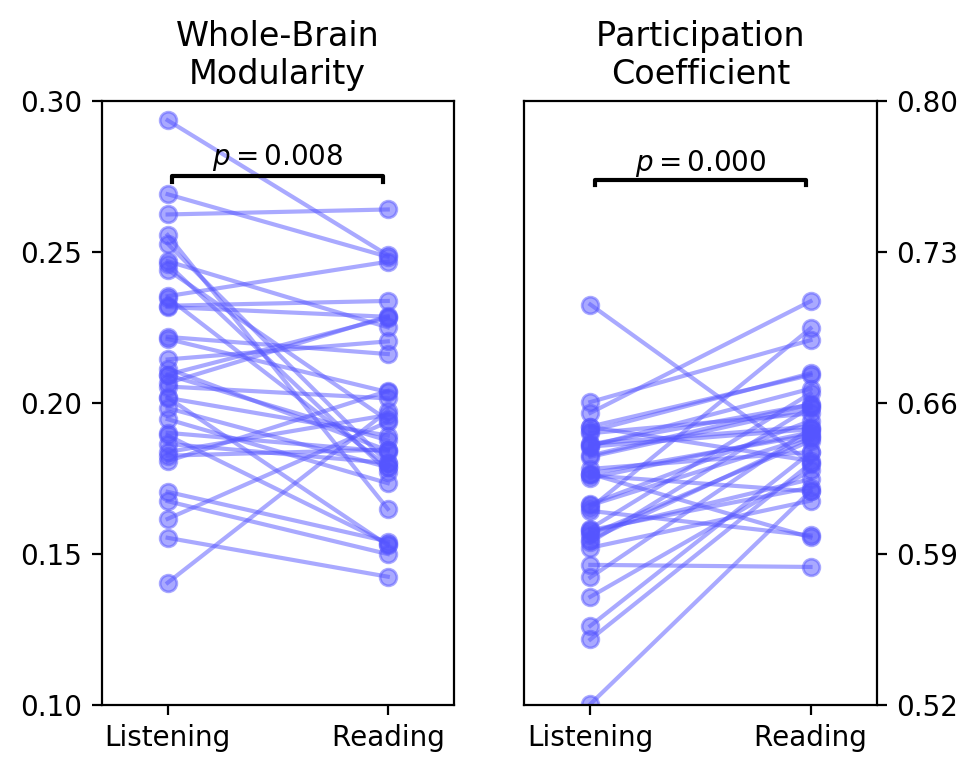
\includegraphics[height=3in]{ch4-modality-graph-theory}
	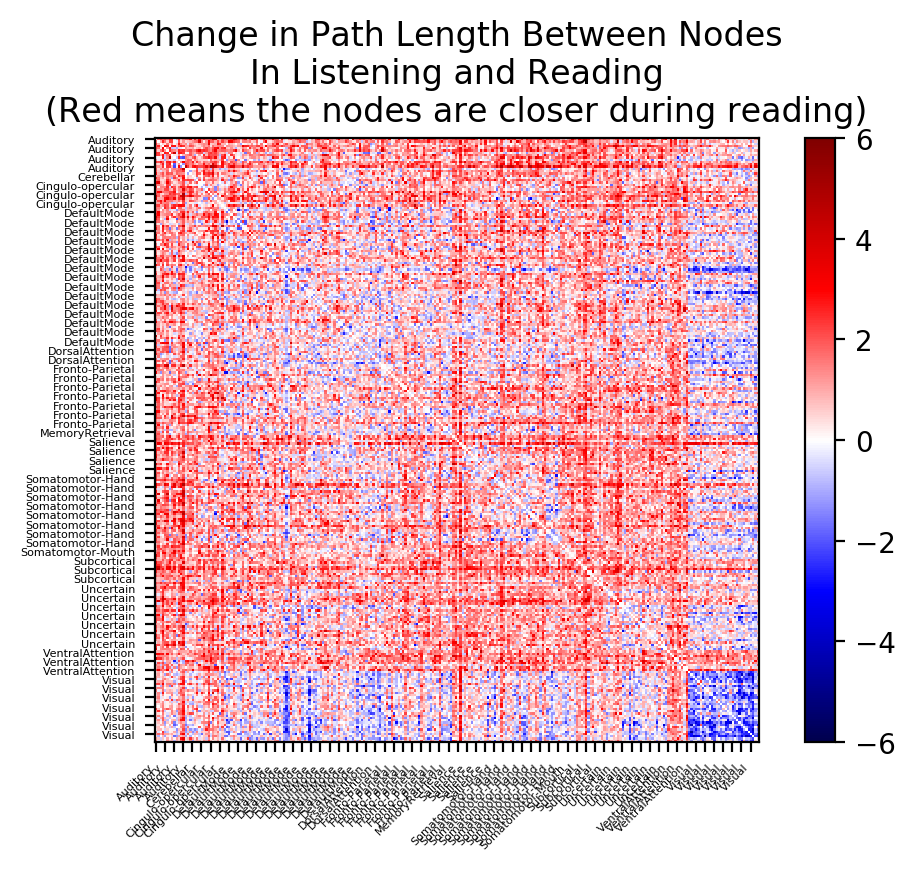
\includegraphics[height=3in]{ch4-modality-node-distance}
    \caption[Reading induces a more integrated network architecture than listening]{Reading induces a more integrated network architecture than listening. In terms of modularity and participation coefficient, there is greater integration during reading than listening. The bottom panel displays the changes to the number of steps connecting each node. The large amounts of red reflect the greater global integration seen in reading; the blue patches represent a reduction in modularity within visual networks especially.}
	\label{fig:ch4-modality-graph-theory}
\end{figure}


\subsection{Network similarity results}

We next investigated whether different individuals evoked language-architectures that were similar to each other. For each pair of participants and modality of presentation, we calculated the IOU between their whole-brain networks. We found that subject connectomes were much more similar when comparing ``listening'' connectomes than when comparing ``reading'' connectomes ($t = 53.190$, $p < 0.001$). Additionally, we found that subjects with the highest mean similarity overall were also more similar to other high-similarity subjects, suggesting that they are each approximating a common architecture during the comprehension process (see top panel of Figure \ref{fig:ch4-modality-network-similarity}).

\begin{figure}[t!]
	\centering
	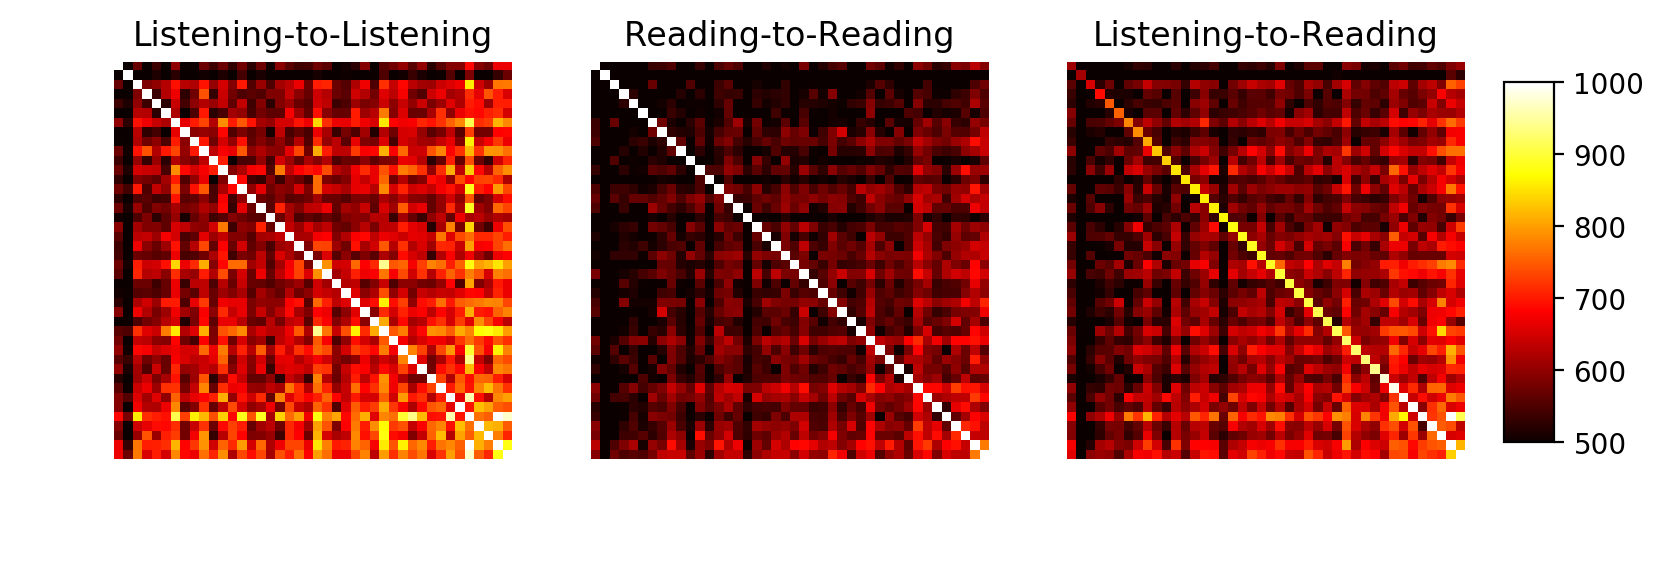
\includegraphics[width=5.5in]{ch4-modality-network-similarity}
	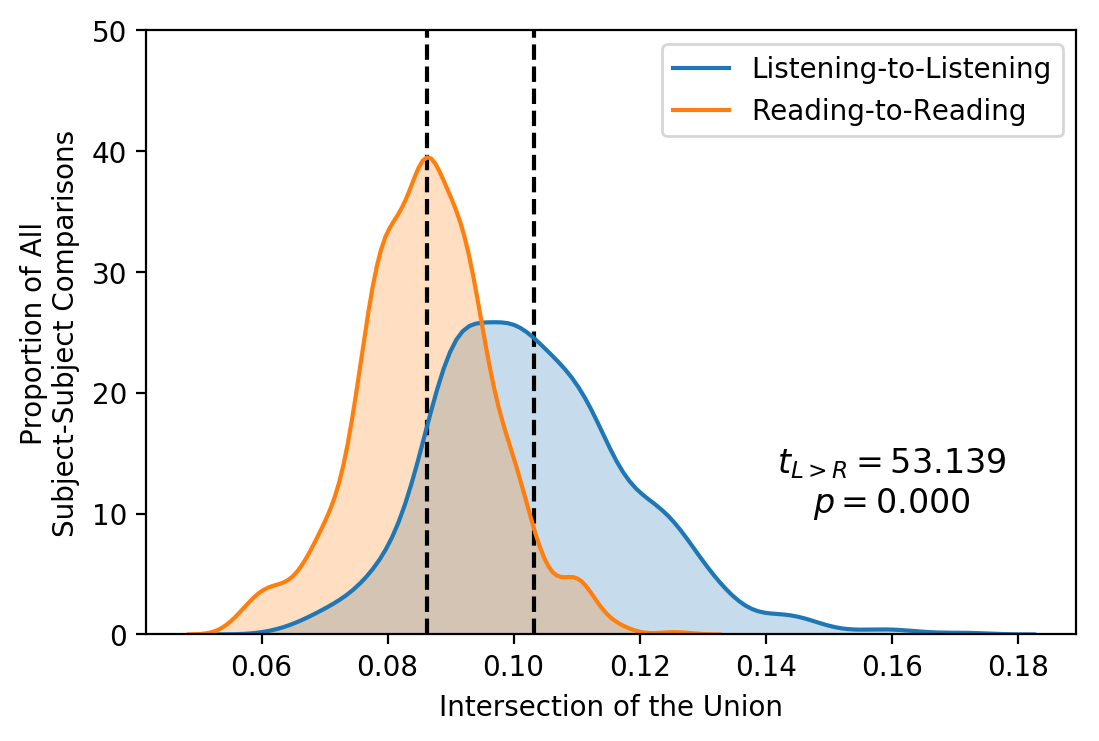
\includegraphics[width=5in]{ch4-similarity-condition-histogram}
    \caption[Network similarity across subjects in listening and reading.] {Distribution of subject similarity values in listening and reading. When comparing participant networks, there is greater similarity in listening than there is in reading (bottom). Furthermore, subjects with high mean similarity were also more similar to each other (top).}
	\label{fig:ch4-modality-network-similarity}
\end{figure}

As readers become more experienced, the expectation is that the task-evoked network architecture for reading would become more similar to that of the ``natural'' listening comprehension system. To test this, we compared each subject's listening network with their reading network then correlated this measure with TOWRE scores (Fig. \ref{fig:ch4-modality-similarity-to-reading}). Better readers did have a higher degree of similarity between the listening and reading networks ($r = 0.408$, $p = 0.007$). Furthermore, we found that reading and listening networks within a subject than between any two subjects ($t = 26.123$, $p < 0.001$). 

\begin{figure}[t!]
	\centering
	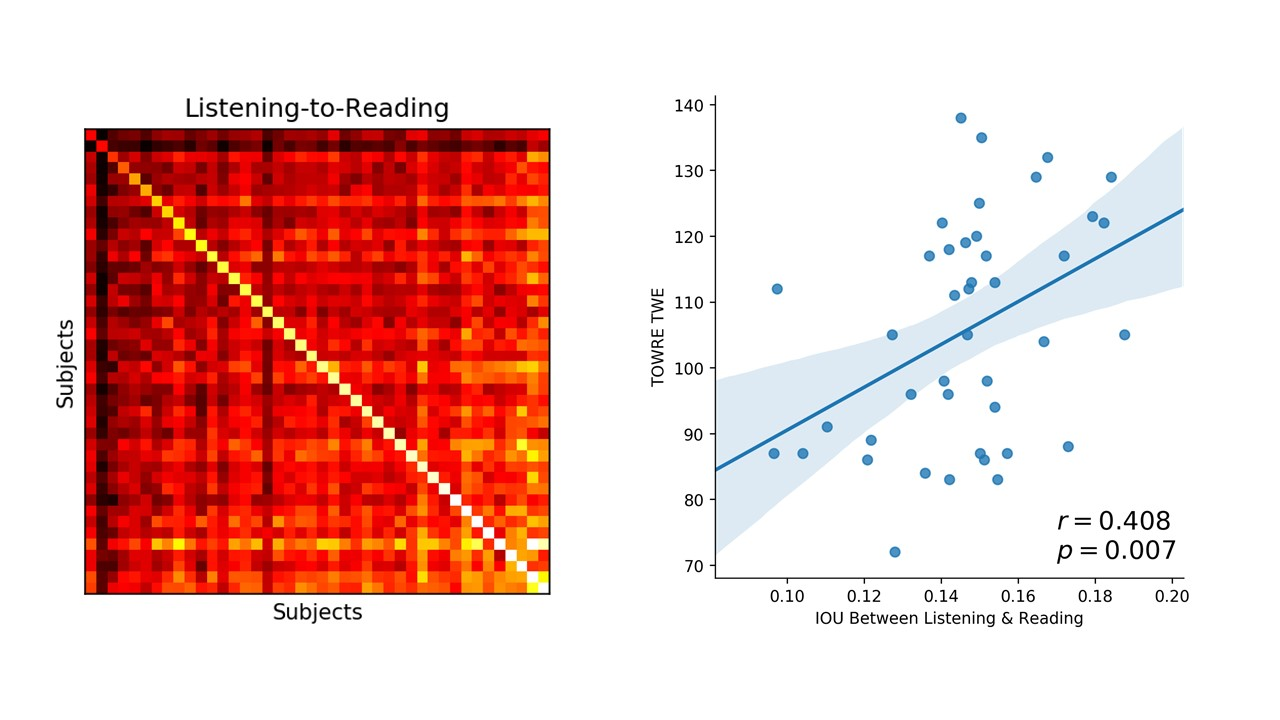
\includegraphics[width=6in]{ch4-listening-to-reading-similarity-skill}
    \caption[Network similarity between listening and reading predicts word efficiency]{Network similarity between listening and reading predicts word efficiency. We compared the listening-evoked network to the reading-evoked networks within each subject and found that it, too, correlated with reading skill.}
	\label{fig:ch4-modality-similarity-to-reading}
\end{figure}

% extended this question to encompass multiple task conditions: would individuals who are better readers have higher similarity between multiple tasks?
We next compared the similarity across all network arrays to determine the degree of variability in architecture within each subject. For each person, we created a similarity matrix describing the shared connections between each of these conditions. Then, we calculated the mean of the shared connections. Figure \ref{fig:ch4-rsn-mean-similarity} shows the distribution of within-subject IOU values across all conditions for each RSN. The global similarity was 0.364, while the highest similarities were among the visual, dorsal attention and memory retrieval conditions; the lowest were in the auditory, ventral attention, subcortical and somatomotor (mouth) regions.

\begin{figure}[t!]
	\centering
	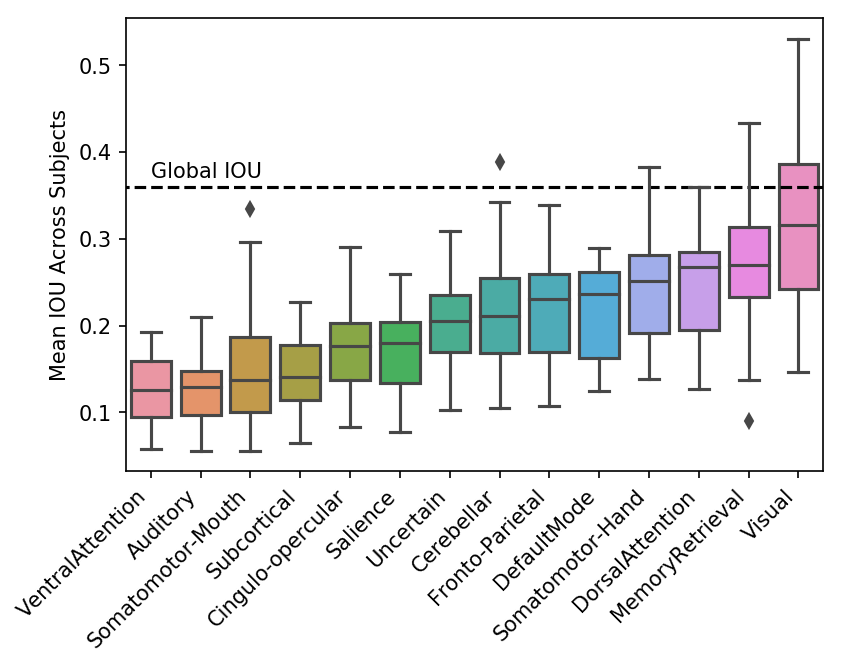
\includegraphics[height=4in]{ch4-rsn-mean-similarity}
    \caption[RSNs share a large degree of similarity]{RSNs share a large degree of similarity. At the global level, the mean similarity among task-evoked networks was higher (0.362) than any individual RSN. Several of the language- and task-oriented RSNs had very low similarity (ventral attention, auditory, somatomotor).}
	\label{fig:ch4-rsn-mean-similarity}
\end{figure}

We next correlated these measures with TOWRE scores. The mean within-subject IOU for the entire connectome (264 nodes) was significantly correlated with the TOWRE Total Word Efficiency standard score ($r = 0.324$, $p = 0.033$). Individual RSNs generally followed this trend, although a few had higher correlations: the ventral attention ($r=0.384$), fronto-parietal ($r=0.370$), salience ($r=0.352$) and default mode ($r=0.346$) networks were slightly greater than the whole-brain IOU. To test whether this was specific to reading skill or more general, we performed the same correlation using the Vocabulary scores from the WASI intelligence test. We found an even stronger correlation between global similarity measures and vocabulary scores ($r = 0.481$, $p < 0.001$), with the trend continuing for the other RSNs. 

\begin{table}[t!]
	\renewcommand{\tabcolsep}{0.09cm}
	\centering
	\begin{tabular}{lll}
\toprule
Resting-State Network & $r_{TOWRE}$ & $r_{WASI-Vocabulary}$ \\
\midrule
Global           & 0.324* & 0.481** \\
VentralAttention  &        0.384* &       0.453** \\
Fronto-Parietal   &        0.370* &       0.498** \\
Salience          &        0.352* &       0.416** \\
DefaultMode       &        0.346* &       0.509** \\
Subcortical       &        0.327* &       0.325*  \\
Somatomotor-Mouth &        0.322* &       0.402** \\
Visual            &        0.316* &       0.456** \\
Cingulo-opercular &        0.307* &       0.271   \\
Auditory          &        0.283 &       0.417**  \\
MemoryRetrieval   &        0.277 &       0.469**  \\
Cerebellar        &        0.267 &       0.346*   \\
DorsalAttention   &        0.261 &       0.464**  \\
Uncertain         &        0.136 &       0.234    \\
Somatomotor-Hand  &        0.119 &       0.285    \\
\bottomrule
\end{tabular}
	\caption[Correlation values between shared connectivity and cognitive skill]{Correlation values between shared connectivity and cognitive skills. Individual RSNs generally followed the global trend, with the exception of the unclassifiable and somatomotor (hand) RSNs.}
	\label{table:ch4-rsn-similarity-to-reading}
\end{table}

\section{Discussion}

% Recap study rationale and results
This study addressed two questions: how does task-evoked network architecture vary between two highly similar tasks, and how do individual differences in this variability relate to cognitive skills? We covered differences between reading and listening at the level of activitation, global network measures and network similarity. At all levels, we found a high degree of similarity between listening and reading relative to the other conditions, but with reading eliciting more more integration across RSNs and more variability between subjects. We found that the degree of similarity between listening and reading task-evoked networks was related to reading skill; the degree of similarity between all of the conditions, in fact, was related to reading skill. The results provide further support that variability in network architecture is not associated with increased cognitive performance. Rather, it seems to be the case that the ``evoked'' networks approximate a baseline architecture that is suprisingly stable across task demands.

% Modality differences: activation
Reading and listening elicited a similar activation profile with many overlapping areas. This is consistent with previous research and theoretical models suggesting that, after the act of word recognition, reading and listening share a common supramodal core set of processing areas \citep{Rueckl2015, Hoover1990, Price2012}. However, there were some important differences. The first was the finding of greater activity during reading along several shared language-related areas, including the temporo-parietal junction and inferior frontal gyrus. The greater activation here likely represents more effortful processing: in developing readers, there is an elevated BOLD signal for reading compared to listening \citep{Berl2011}. This elevation is also true for individuals with dyslexia who will sometime exhibit greater activation in reading-related areas compared to typically developing children \citep{Pugh2000}. 

% Dorsal attention network
The other meaningful difference is the deactivation of the dorsal attention network during reading, relative to listening. The dorsal attention network has a push-pull relationship with the ventral attention and salience networks. Because the ventral attention network is so heavily engaged during reading (viz. Chapter 3), it is likely that this reduction in DAN activity is a response to it. The DAN is closely connected to language areas including the visual word form area \citep{Bouhali2014}, but also plays a major role in guiding top-down attention, and is closely related to other executive RSNs such as the fronto-parietal \citep{Vogel2014}. Vogel and colleagues found that reading ability in typical children and adults (including decoding and passage comprehension ability) predicted increased correlations between the visual word form area and the DAN \citep{Vogel2012a}. That the deactivation of the DAN (and activation of the VAN) are present in a contrast of the two skills suggests that these attention processes are unique to reading and not general to language comprehension. To our knowledge, this is the first report of this.

% Significance of graph theory results - greater integration globally driven by visual ``de-clustering''

% Higher similarity among listening networks
Speech comprehension is ``natural'', in the sense that most everyone learns to understand language regardless of their educational environment. The greater similarity values observed when comparing the listening-evoked networks across participants may reflect the more practiced nature of speech. On the other hand, the greater variability in the reading-evoked network might be indicative of the additional interactions necessary in reading: guided control of eye movements, visual processing, additional engagement of the attention systems \citep{Mattingly1971}. There are also differences in what is encoded in speech and text.  Speech contains overt clues about the speaker, such as tone and prosody, and these can convey additional non-linguistic meaning for the listener. Reading could be considered a more purely linguistic act. Reading may thus allow more room for self-generated situation models and more independent direction of thought. 

% Relationship with similarity
As readers become more experienced, the expectation is that the task-evoked network architecture for reading would become more similar to that of the intrinsic listening comprehension system. It is thus expected that greater overlap between the two systems would be correlated with reading skill, as it was. Once again, each individual RSN was broadly representative of the global trend, but there were a few of particular note. Similarity of structure in the fronto-parietal and default mode networks were the only RSNs that outperformed the global IOU in both correlations with cognitive skills. It could be argued that these two represent the two core higher-order RSNs. High similarity in both implies that they are anti-correlated, once again touching upon the segregation hypothesis. The two RSNs that had no correlation with either measure were the ``uncertain'' nodes -- nodes whose connectivity profiles were too variable to assign to an RSN -- and the somatomotor (hand) RSN, whose connectivity may have been strongly influenced by the tapping task throughout the scans. 

%
The overarching result is that variability in task-evoked network architecture, whether it is between language tasks, simple sensory tasks or resting state, is anti-correlated with cognitive performance. Although alterations to the intrinsic organization are inevitable when performing a task, the degree of reorganization appears to be related to the task difficulty -- or at least the extent of cognitive functions employed -- with reading representing the most taxing model investigated by us. We have also seen that differences in the network architecture are robust within individuals: the correlations with reading have held across a number of different network measures. But how and when do they change? Does the relationship with reading hold true throughout the lifespan? We tackle this question in the next chapter. 